\begin{center}
    {\LARGE \textbf{Parte V}}\\[6pt]
\end{center}
\vspace{4pt}\hrule\vspace{10pt}

\maketitle

\section*{Ítem 22}

\begin{table}[H]
\centering
\caption{Estadísticos cíclicos por país}
\begin{tabular}{lcccccc}
\toprule
País & Grupo & R2 & R3 & R4 & R5 & R6 \\
\midrule
USA & Desarrollado & -0.232 & -0.212 & 0.530 & 0.796 & 0.687 \\
DEU & Desarrollado & -0.022 & -0.008 & 0.270 & 1.637 & -0.265 \\
CHN & Emergente & 0.082 & 0.104 & 0.123 & 0.916 & 0.838 \\
PER & Emergente & -0.249 & -0.058 & 0.444 & 0.665 & 0.564 \\
CHL & Emergente & -0.306 & -0.271 & 0.501 & 0.707 & 0.124 \\
KOR & Emergente & -0.627 & -0.642 & 0.396 & 1.773 & 0.612 \\
TUR & Emergente & -0.393 & -0.461 & 0.399 & 0.966 & 0.810 \\
\bottomrule
\end{tabular}
\end{table}

\begin{figure}[H]
\centering
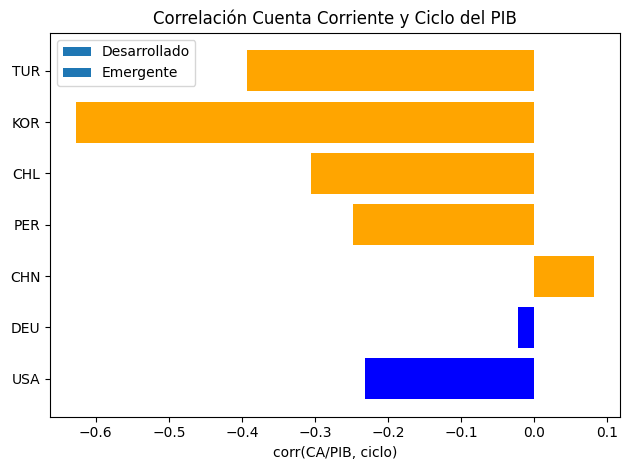
\includegraphics[width=0.8\textwidth]{grafico_item22.png}
\caption{Correlación entre cuenta corriente y ciclo del producto por país}
\end{figure}

\section*{Ítem 23}

\subsection*{(a)}
R2 se cumple en todos los países menos China, pues este último tiene una corr con CA positiva (+0.082). El promedio (en valor absoluto) de R2 en economías desarrolladas es de 0.127, mientras que en emergentes es 0.331. Esto confirma que la CA es más cotracíclica en economías emergentes.
Si se puede ver un patrón, en las economías emergentes, la mayor contraciclidad en la CA indica que la inversión es la referente en los ajustes ante shocks. En cambio, en economías desarrolladas se muestra un suavizamiento del consumo. Esto hace sentido pues las economías desarrolladas tienen un mejor acceso a los sistemas financieros internacionales, que permite tener un endeudamiento prolongado.


\subsection*{(b)}
R6 no se cumple para Alemania (tiene un valor -0.265). Chile tiene un R6 positivo pero bastante bajo.
Cuando S-I es bajo, el ahorro doméstico y la inversión no se vinculan fuertemente. Esto significa que el país puede ahorrar en el exterior o financiar su inversión con capital del exterior. Por lo tanto, el valor bajo de S-I si sugiere que el país esté más integrado en el sistema financiero internacional (y mayoe movilidad de capitales).


\subsection*{(c)}
R5 falla para Alemania (1.637) y Corea (1.773), eso indica que la inversión es más volatil que el consumo. En los demás países se da el caso contrario. Las economías que muestran el comportamiento más volatil en el consumo suelen ser emergentes (es curioso que esté EE.UU.), pues estas presentan mayores problemas para suavizar el consumo, puede ser por el limitado acceso al crédito, y su sensibilidad es mayor ante shocks.


El primer país que no coincide con la teoría inicial es EE.UU., esto puede deberse a lo relevante que es el dólar a nivel mundial como moneda de reserva. Esta gran demanda por la moneda da un buen espacio a EE.UU. para financiar sus desequlibrios externos facilmente.
El segundo país que no coincide con la teoría es Chile. Este país usa sus fondos soberanos para obtener una política contracíclica y suavizar la inversión pública. Además, es un país afectado por los shocks detérminos de intercambio (precio del cobre mayormente), esto hace que el ingreso nacional tenga una mayor fluctuación y el conusumo sea impactado.


\section*{Ítem 24}

En la economía sin inversión no existe acumulación, los agentes ahorran en momentos positivos y desahorran en una recesión. Por lo tanto, se puede observar comportamiento procíclico en cuanto a la CA. Asimismo, va de acorde al comportamiento de R1

En la economía con inversión, en cambio, cuando hay un shock de productividad, por ejemplo, y la demanda por capital (para invertir) aumenta, lo que genera deficits externos y, por consecuencia, reducir la CA (contracíclica). Esto va de acorde al comportamiento de R2.

R1 se asocia con la CA procíclica (aquí se da el suavizamiento de consumo) y R2 se asocia con la CA contracíclica (acumulación de capital), por lo tanto, el canal que se encuentra apagado en una economía de dotaciones es el de inversión (acumulación de capital).

corr(CA/PIB, ciclo) con inversion = -0.033
corr(CA/PIB, ciclo) sin inversion = +0.318

\begin{figure}[H]
\centering
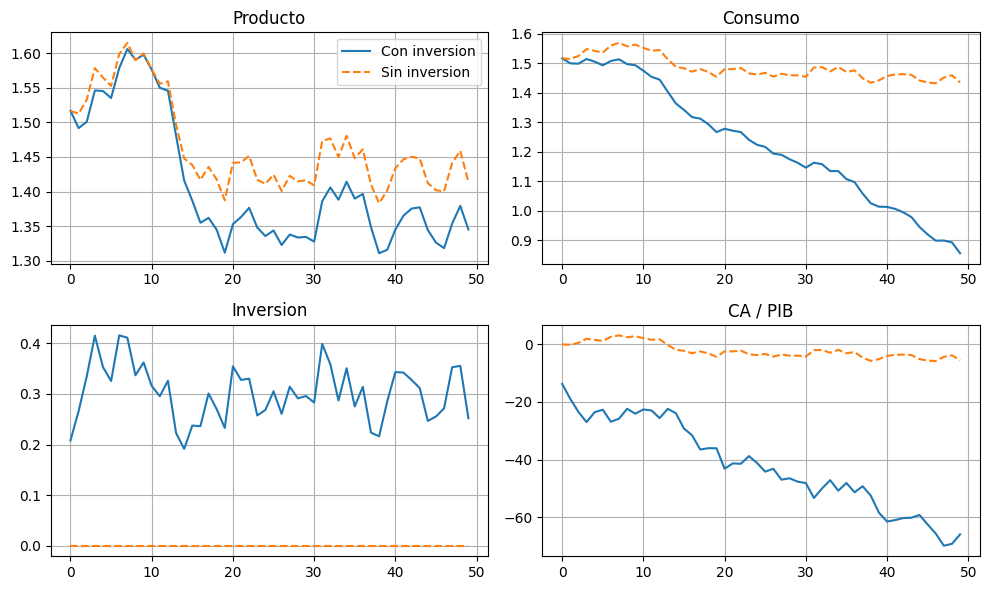
\includegraphics[width=0.8\textwidth]{grafico_item24.png}
\caption{Comparación de dinámicas con y sin inversión}
\end{figure}

\section*{Ítem 25}

\begin{table}[H]
\centering
\caption{Efectos de cambios paramétricos sobre inversión y cuenta corriente}
\begin{tabular}{cccc}
\toprule
Parámetro & Cambio & $\Delta I$ & $\Delta CA$ \\
\midrule
$\rho$ & $\uparrow$ & $\uparrow$ & $\downarrow$ \\
$\alpha$ & $\uparrow$ & $\uparrow$ & $\downarrow$ \\
$r^*$ & $\uparrow$ & $\downarrow$ & $\uparrow$ \\
$\sigma_{\epsilon}$ & $\uparrow$ & $\uparrow$ & $\downarrow$ \\
$\beta$ & $\uparrow$ & $\uparrow$ & $\uparrow$ \\
\bottomrule
\end{tabular}
\end{table}

\begin{table}[H]
\centering
\caption{Intuición económica de los cambios paramétricos}
\begin{tabular}{p{2cm} p{11cm}}
\toprule
Parámetro & Intuición \\
\midrule
$\rho$ & Como shock es más persistente, el retorno esperado de capital es elevado y se incentiva a invertir hoy, esto incrementa el déficit externo \\

$\alpha$ & Mayor peso de capital eleva la productividad marginal, aumenta inversion y mayor déficit en CA \\

$r^*$ & Mayor costo de financia. desincentiva inversión y reduce endeudamiento externo, por lo que CA aumenta\\

$\sigma_{\epsilon}$ & Shocks generan mayor fluctuacion en inversion, se amplifican los deficits y superavits externos \\

$\beta$ & Agentes más pacientes ahorran más, reduce la necesidad de financiarse y modera el deficit de CA \\
\bottomrule
\end{tabular}
\end{table}


\section*{Ítem 26}

\subsection*{Paso 1}

Se aumentó $\rho$, $\alpha$ y $\sigma_\epsilon$, y se redujo $r^*$ para mejorar los momentos del modelo.

\begin{table}[H]
\centering
\caption{Comparación de momentos: modelo base vs calibrado}
\begin{tabular}{lccc}
\toprule
Momento & Base & Calibrado \\
\midrule
corr(CA, ciclo) & 0.012 & 0.011 \\
corr(I, ciclo) & 0.634 & 0.551 \\
$\sigma(I)/\sigma(C)$ & 0.012 & 0.059 \\
\bottomrule
\end{tabular}
\end{table}

\subsection*{Paso 3}

Simular-economía es una versión muy simple de una economia abierta. El paper incorpora shocks en los términos de cambios (como el cobre) que afectan directamente en la CA. También desgrega el gasto, lo que mueve bastante la dinámica entre el consumo y la inversion. Además, el paper incorpora un ambiente de dinámica inflacionaria y política monetaria que no se encuentran en este sencillo modelo.  Los criterios del paper permiten modelar de forma más empírica sin la necesidad de ajustar demasiado los parámetros.

\end{document}